\chapter{Opzetten van de Cassandra cluster}
\label{ch:cassandra_cluster}

\section{Apache Cassandra}
Om de cluster op te zetten werd geopteerd om gebruik te maken van virtuele machines, die geconfigureerd werden met Vagrant.

In een eerste poging om een werkende Cassandra cluster te bekomen werd op elke Vagrant machine Cassandra 3.3, op het moment van dit onderzoek de meest recente versie, geïnstalleerd.
Nadat dit gebeurd was, dienden nog enkele stappen voltooid te worden om een werkende cluster te bekomen \citep{DataStax2016}.
Deze configuratie gaf echter veel problemen.
Cassandra werd na enkele bewerkingen telkens onbruikbaar en gaf de volgende foutmelding weer: ''could not access pidfile for Cassandra''.
Een eerste oplossing voor dit probleem was om ervoor te zorgen dat de user 'cassandra' toegang had tot de pidfile, wat namelijk niet het geval was doordat de installatie van Cassandra werd uitgevoerd door de Vagrant setup.
Maar ook dit leverde weinig resultaat op.
Wel moet opgemerkt worden dat de installatie van Cassandra zelf geen problemen met zich meebracht.
Voor de aanpassing van de configuratiefile van Cassandra werkte deze perfect op iedere node.

\section{DataStax OpsCenter}

Uiteindelijk werd ervoor geopteerd om gebruik te maken van OpsCenter omdat dit een gemakkelijke manier is om snel een Cassandra cluster te bekomen en omdat er ook goede mogelijkheden tot observeren van de database aanwezig zijn.
Er werd voor OpsCenter community edition 5.2.4 gekozen.
Bij deze versie diende Cassandra 2.1.11 gebruikt te worden \citep{Cantoni2016}.

De setup bestaat uit één master node waarop het OpsCenter runt en verder uit drie slave nodes waarop de uiteindelijke Cassandra database komt te runnen.
Na de NAT router van Oracle Virtual Box werd een privaat netwerk opgezet opdat deze machines met elkaar zouden kunnen communiceren.
Hiervoor moest iedere machine een uniek ip-adres krijgen binnen het netwerk en moest de file /etc/hosts op iedere node aangepast worden.
De scripts hiervoor kunnen in bijlage B teruggevonden worden.

Eenmaal de virtuele machines correct geconfigureerd waren, kon overgegaan worden tot de eigenlijke installatie van Cassandra.
Zoals eerder vermeld, werd hiervoor gebruik gemaakt van het OpsCenter.
Daarom werd op de master node naar 'localhost:8888' gesurft om de installatie te kunnen  starten.
Op de pagina werden verschillende opties aangeboden en hier werd voor de optie 'brand new cluster' gekozen.

In het volgende venster wordt om verschillende zaken gevraagd.
Tabel \ref{tab:cas_conf} en figuur \ref{fig:cas_conf_1} geven weer hoe dit venster werd ingevuld.

\begin{table}[H]
  \begin{tabular}{|l|l|}
  \hline
  Property Name & Waarde \\
  \hline
  \hline
  Cluster Name & BP Cluster \\
  \hline
  Type & local \\
  \hline
  Package & datastax community 2.1.11 \\
  \hline
  Enpoint Snitch & GossipingPropertyFileSnitch \\
  \hline
  Username en password & vagrant/vagrant\\
  \hline
  Local Node Credentials & cassandra-node-1, cassandra-node-2, cassandra-node-3 \\
  \hline
  \end{tabular}
  \caption{Configuratie van de Cassandra Cluster}
  \label{tab:cas_conf}
\end{table}

\begin{figure}[H]
  	\centering
    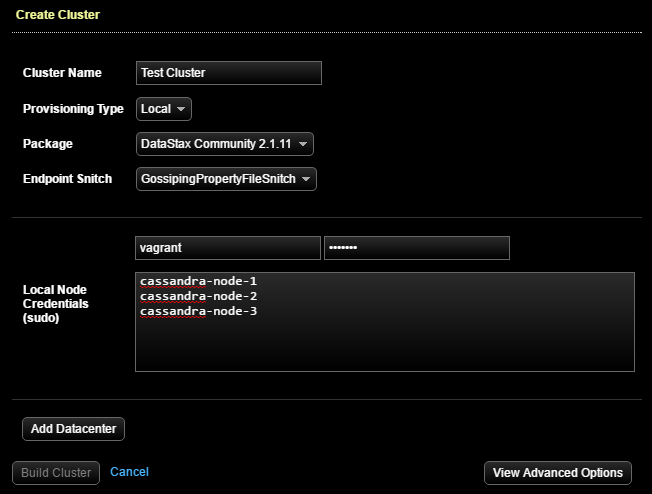
\includegraphics[width=0.5\textwidth]{img/4_installatie_cassandra/1_Configuration_part_1}
    \caption{Cassandra: Instellingen deel 1}
    \label{fig:cas_conf_1}
\end{figure}

Hier moest een datacenter toegevoegd worden.
Hierbij is er een vrije keuze voor de naam van het datacenter en zijn de node properties het ip-adres van de slave nodes (Figuur: \ref{fig:cas_conf_2}).

\begin{figure}[H]
  	\centering
    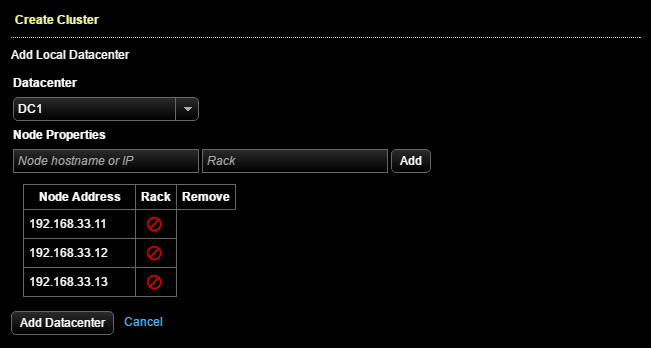
\includegraphics[width=1.0\textwidth]{img/4_installatie_cassandra/1_Configuration_part_2}
    \caption{Cassandra: Instellingen deel 2}
    \label{fig:cas_conf_2}
\end{figure}

Eenmaal de datacenters toegevoegd zijn, kan er verder gegaan worden.
Bij het drukken op de knop 'build cluster' wordt verder nog gevraagd om de fingerprints van de nodes te accepteren.

Hierna begint OpsCenter met de installatie van de Cassandra cluster (Figuur: \ref{fig:cas_install}).
Deze installatie nam enige ogenblikken in beslag.
De eerste keer kwam er een fout voor omdat er niet genoeg werkgeheugen was toegekend aan de slave nodes.
In de setup die hier gebruikt werd, werd het minimum aanvaarde geheugen, nl 2GB, gegeven aan de slave nodes.
Samen met Cassandra wordt ook de DataStax agent mee geïnstalleerd opdat het OpsCenter zou kunnen communiceren met iedere node.

\begin{figure}[H]
	\centering
	\begin{subfigure}{.49\textwidth}
  		\centering
  		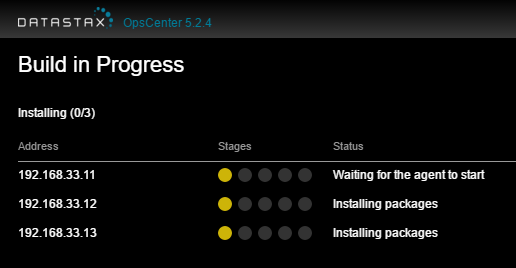
\includegraphics[width=.9\linewidth]{img/4_installatie_cassandra/1_Configuration_part_4}
  		\caption{Deel 1}
	\end{subfigure}
	\begin{subfigure}{.49\textwidth}
  		\centering
  		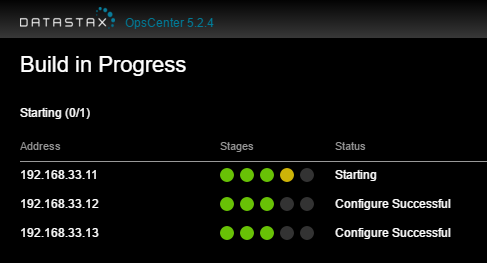
\includegraphics[width=.9\linewidth]{img/4_installatie_cassandra/1_Configuration_part_5}
  		\caption{Deel 2}
	\end{subfigure}
	\begin{subfigure}{.49\textwidth}
  		\centering
  		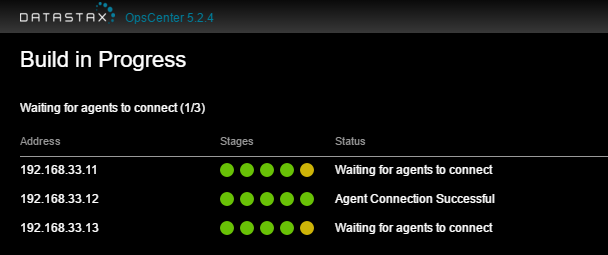
\includegraphics[width=.9\linewidth]{img/4_installatie_cassandra/1_Configuration_part_6}
  		\caption{Deel 3}
	\end{subfigure}
	\caption{Installatie van Cassandra door OpsCenter}
	\label{fig:cas_install}
\end{figure}

Na de installatie komt men terecht in het Dashboard van OpsCenter (Figuur \ref{fig:cas_opscenter_tour_dashboard}).
Hierin worden een aantal zaken weergegeven zoals: de gezondheid van de cluster, het aantal write requests, de write request latency\dots
Hier kunnen nog meer grafieken aan toegevoegd worden door de knop 'add graph' te gebruiken.
In het tabblad 'nodes' kan de gezondheid van de cluster bekeken worden, net zoals gezien kan worden hoe de data verdeeld zit over de cluster.
Deze informatie kan in ringvorm, zoals in figuur \ref{fig:cas_opscenter_tour_nodes} weergegeven wordt, of in een lijst weergegeven worden.

\begin{figure}[H]
	\centering
	\begin{subfigure}{.49\textwidth}
		\centering
		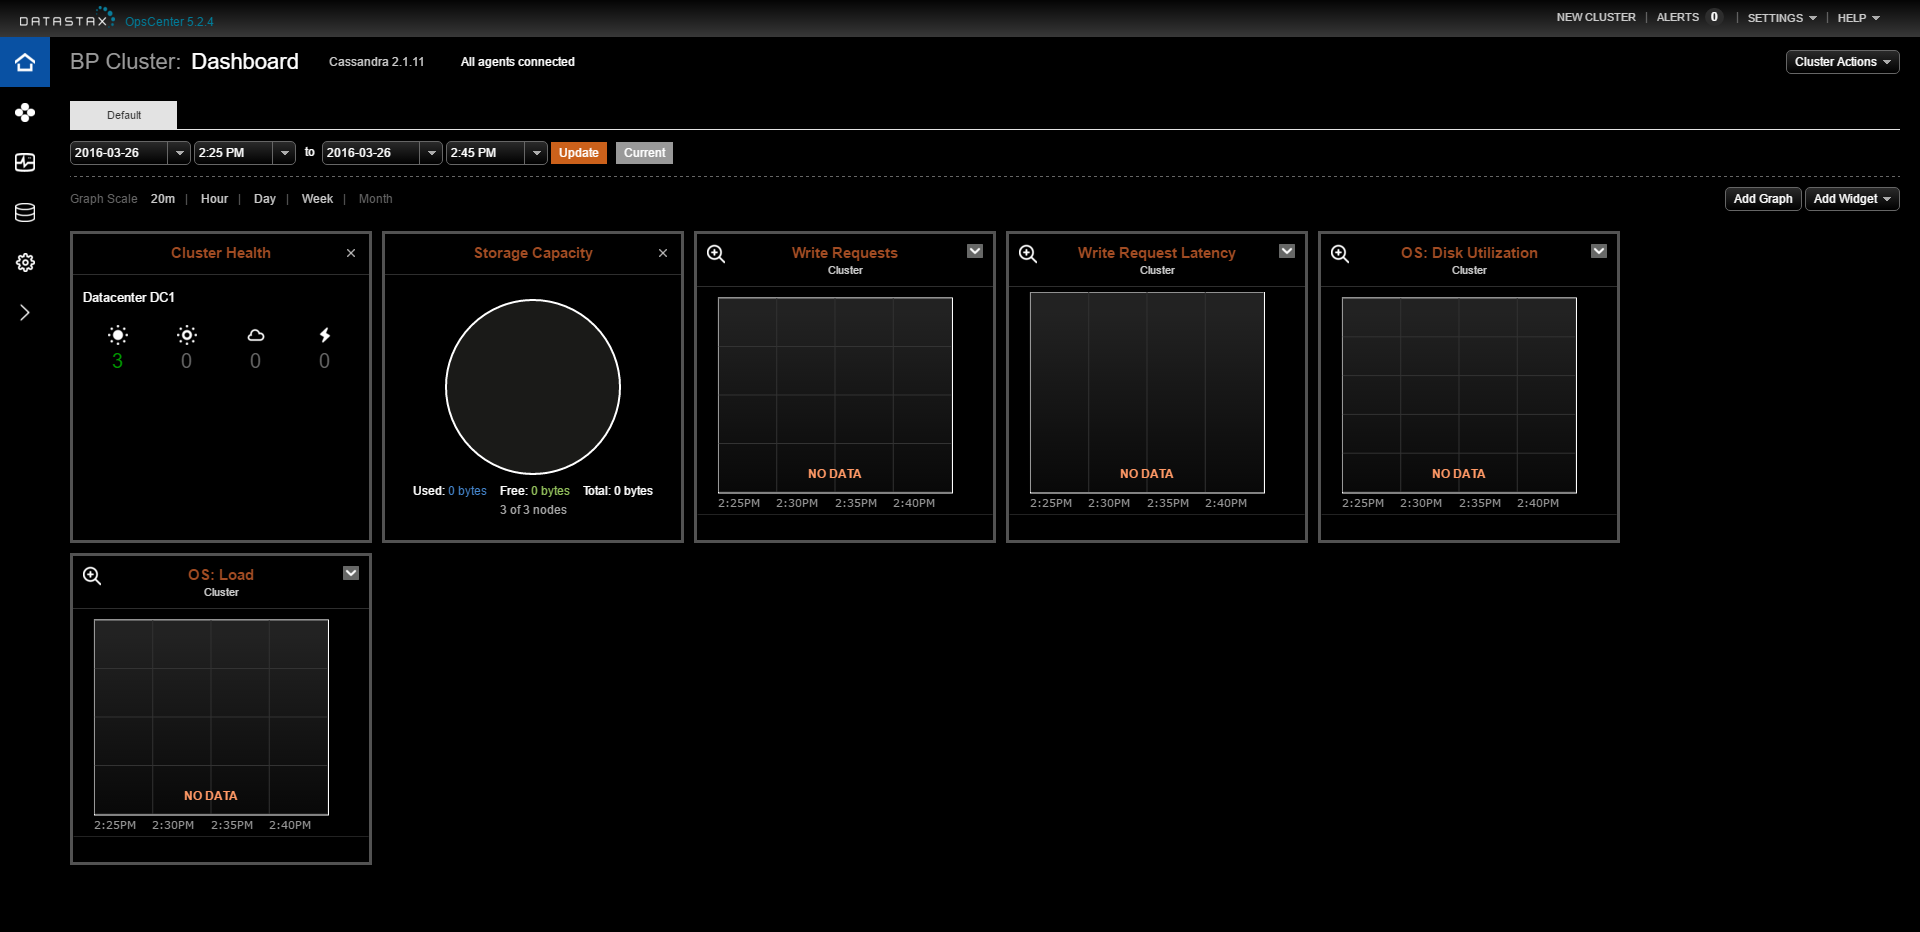
\includegraphics[width=.99\linewidth]{img/4_installatie_cassandra/2_Tour_1_Dashboard}
		\caption{Tabblad dashboard}
		\label{fig:cas_opscenter_tour_dashboard}
	\end{subfigure}
	\begin{subfigure}{.49\textwidth}
		\centering
		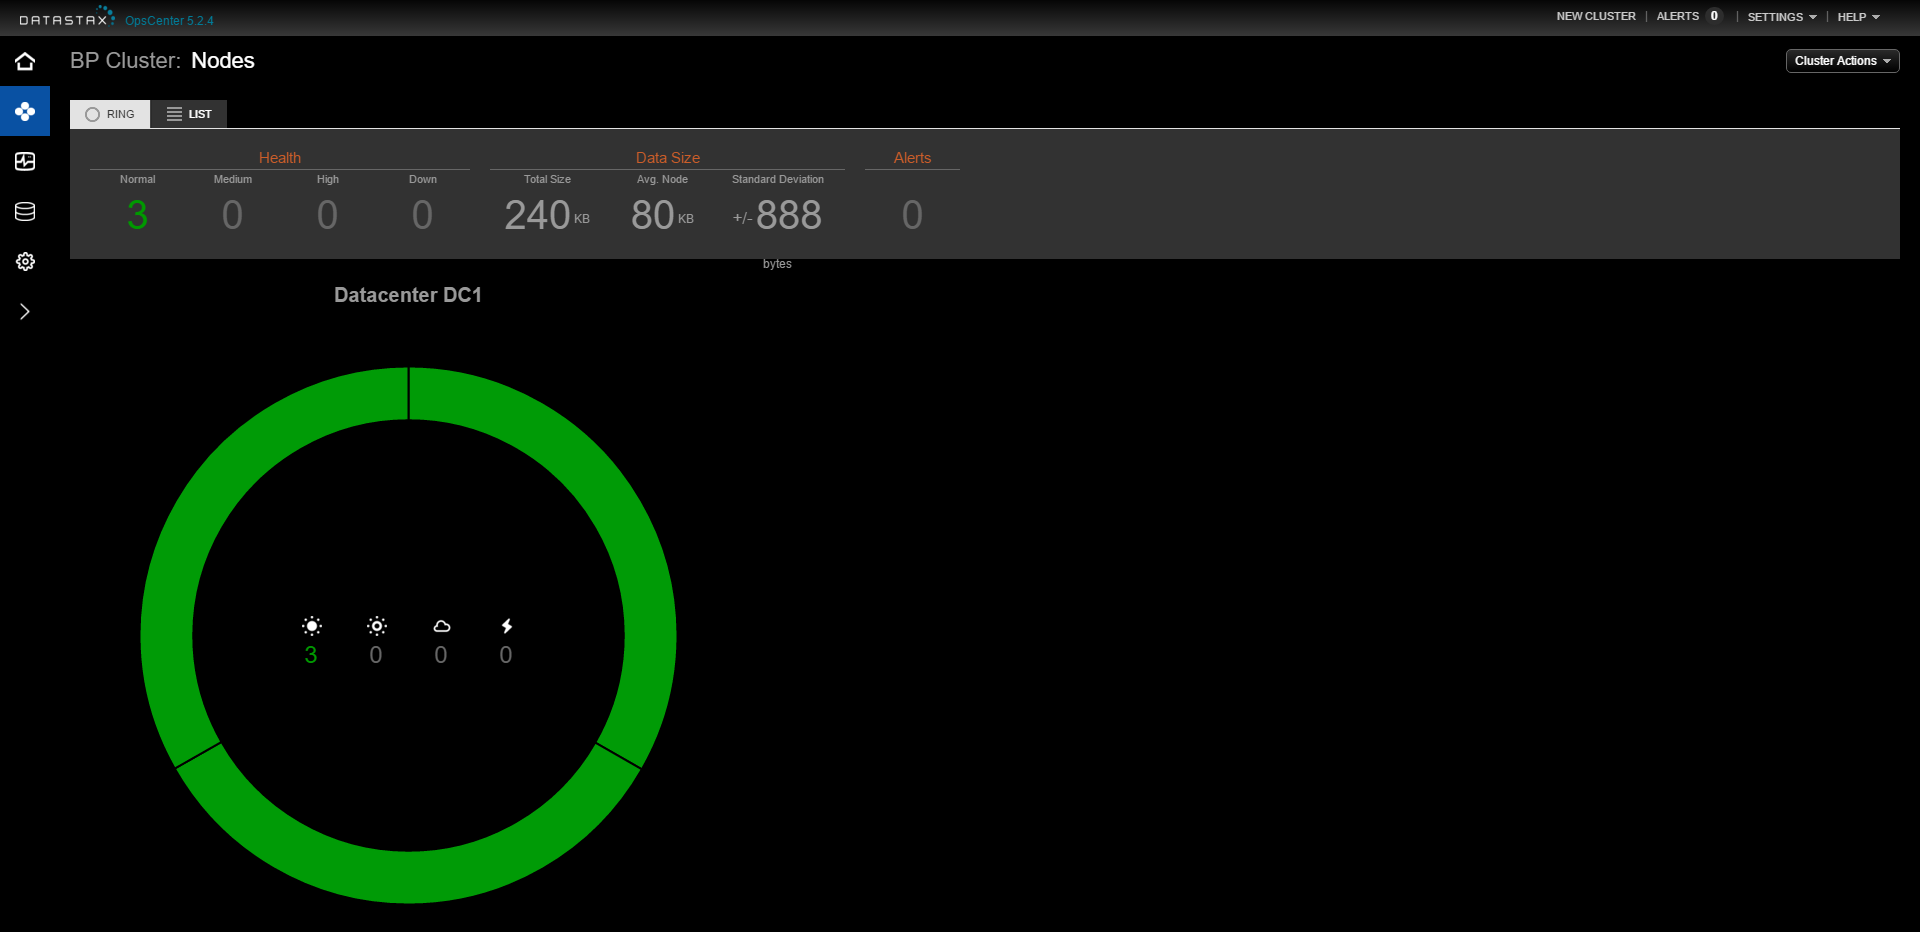
\includegraphics[width=.99\linewidth]{img/4_installatie_cassandra/2_Tour_2_Nodes}
		\caption{Tabblad nodes: ring}
		\label{fig:cas_opscenter_tour_nodes}
	\end{subfigure}
	\caption{Rondleiding in OpsCenter}
	\label{fig:cas_opscenter_tour}
\end{figure}

Cassandra biedt zelf ook een tool aan die deze monitoring uitvoert: ''nodetool''.
Om te bekijken of de installatie goed gelukt is, kan men via ssh inloggen op één van de nodes van de cluster en hier 'nodetool status' laten lopen (Figuur \ref{fig:cas_nodetool}).
Als men met nodetool de status opvraagt, krijgt men eveneens alle nodes in de cluster te zien, samen met de hoeveelheid data die ze bevatten en hoeveel procent deze data inneemt van alle data die op de cluster aanwezig is.

\begin{figure}[H]
	\centering
	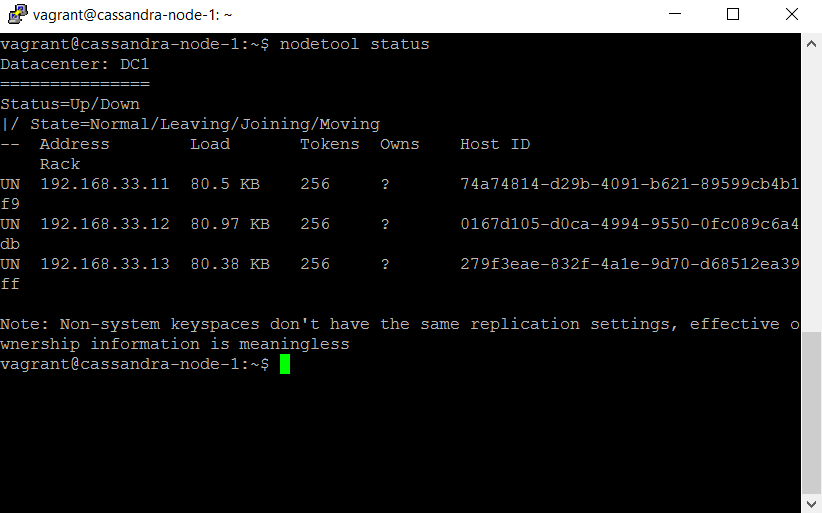
\includegraphics[width=1.0\textwidth]{img/4_installatie_cassandra/3_Node_setup}
	\caption{nodetool}
	\label{fig:cas_nodetool}
\end{figure}

\section{Toevoegen van een node}
Het proces voor de toevoeging van een node is quasi gelijk aan het opzetten van de cluster.
Hierbij dient men in het OpsCenter bij het menu 'cluster actions' voor de optie 'add node' te kiezen (Figuur \ref{fig:cas_add_node_1}).
Hier wordt een vierde node aan de cluster toegevoegd.
Net zoals bij de installatie van de cluster wordt het scherm, waarin de aanmeldgegevens voor de gegeven node gevraagd worden, nog eens weergegeven (Figuur \ref{fig:cas_add_node_2}). 
Via de knop 'Add/Expand Datacenter' kan men op dezelfde manier nodes toevoegen aan het bestaande datacenter die tijdens de installatie werd aangemaakt.
Bij het bevestigen wordt opnieuw gevraagd om de fingerprint van de node te accepteren en hierna begint de installatie van de software op de node, waardoor de agent en Cassandra geïnstalleerd en geconfigureerd worden.
Na dit alles kan men in het tabblad 'nodes', nu in een lijstvorm, zien dat de nieuwe node is toegevoegd aan de cluster (Figuur: \ref{fig:cas_add_node_3}).

\begin{figure}[H]
	\centering
	\begin{subfigure}{.49\textwidth}
		\centering
		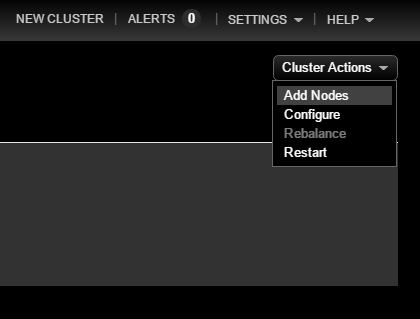
\includegraphics[width=.9\linewidth]{img/4_installatie_cassandra/4_Add_Node_1}
		\caption{Add node}
		\label{fig:cas_add_node_1}
	\end{subfigure}
	\begin{subfigure}{.49\textwidth}
		\centering
		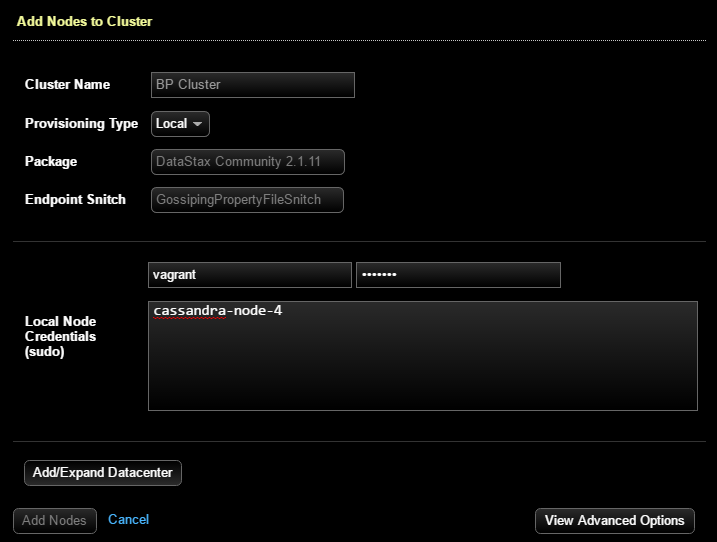
\includegraphics[width=.9\linewidth]{img/4_installatie_cassandra/4_Add_Node_2}
		\caption{Deel 2}
		\label{fig:cas_add_node_2}
	\end{subfigure}
	\begin{subfigure}{\textwidth}
		\centering
		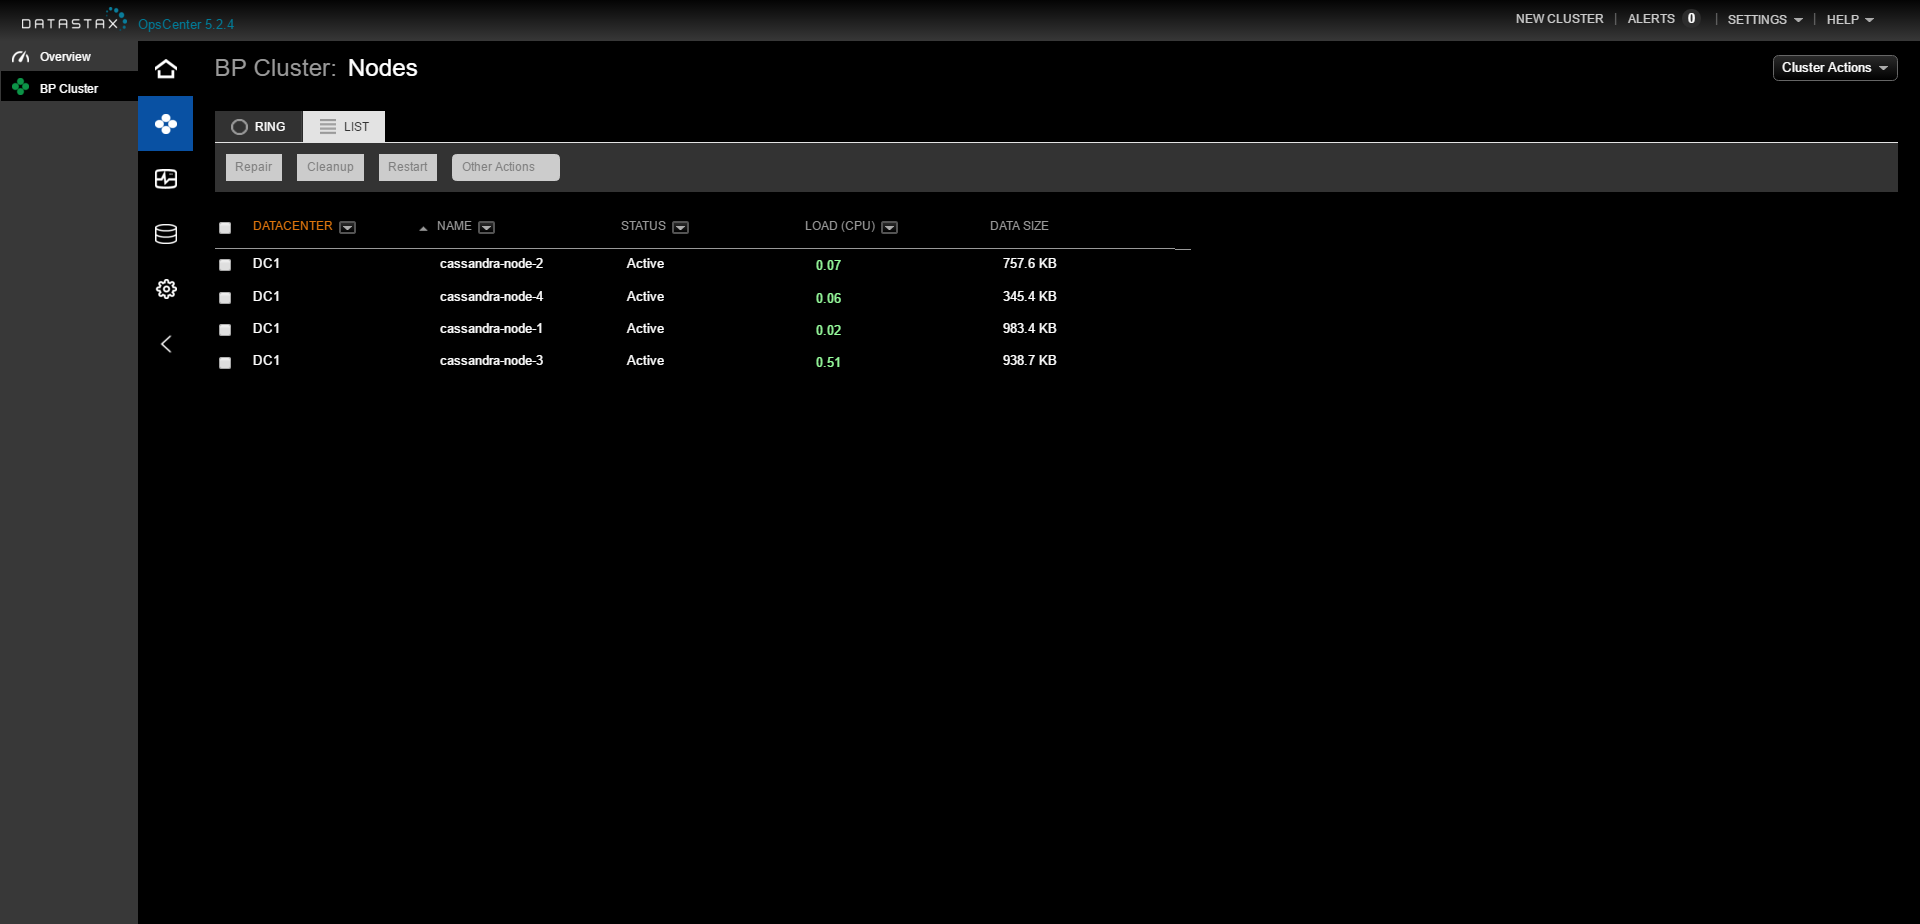
\includegraphics[width=.9\linewidth]{img/4_installatie_cassandra/4_Add_Node_7a}
		\caption{Tabblad node met 4 nodes}
		\label{fig:cas_add_node_3}
	\end{subfigure}
	\caption{Toevoegen van een node via OpsCenter}
	\label{fig:cas_add_node}
\end{figure}

\section{Verwijderen van een node}
Het verwijderen van een node van een Cassandra cluster is - net zoals het toevoegen van een node - zeer eenvoudig.
Binnen het OpsCenter gaat men naar het tabblad nodes en hier selecteert men de node die men wil verwijderen (figuur \ref{fig:cas_rem_1}).

\begin{figure}[H]
	\centering
	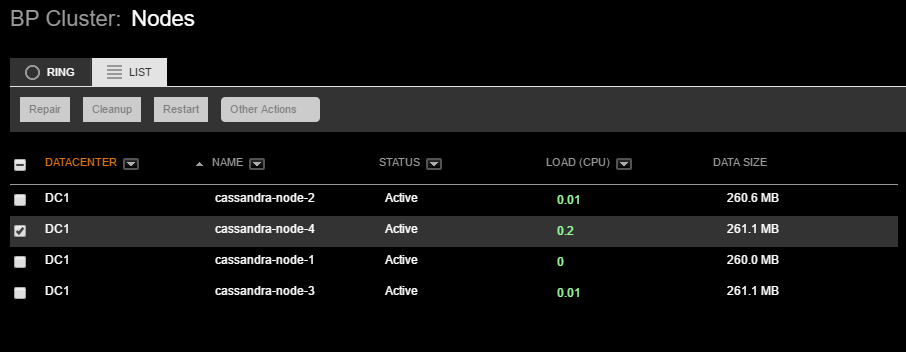
\includegraphics[width=1\textwidth]{img/4_installatie_cassandra/5_Remove_Node_1}
	\caption{Verwijderen van een node: Selecteer de node}
	\label{fig:cas_rem_1}
\end{figure}

Daarna komt men op een volgend scherm terecht (figuur \ref{fig:cas_rem_2}).
Hier kiest men bij de acties voor ''Decommision''.

\begin{figure}[H]
	\centering
	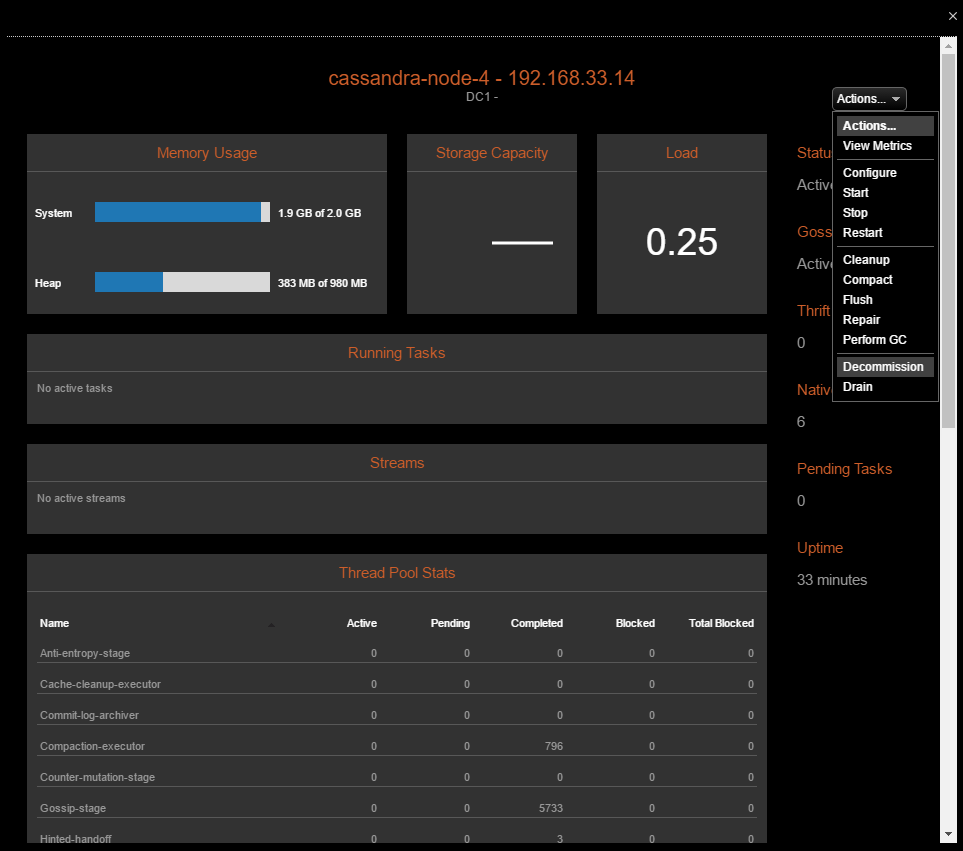
\includegraphics[width=0.8\textwidth]{img/4_installatie_cassandra/5_Remove_Node_2}
	\caption{Verwijderen van een node: Selecteer de node}
	\label{fig:cas_rem_2}
\end{figure}

Voor de node effectief verwijderd wordt, wordt er nog om bevestiging gevraagd.
Hier wordt ook nog meegedeeld dat alle data van de te verwijderen node overgeplaatst zal worden op de andere nodes (figuur \ref{fig:cas_rem_3})

\begin{figure}[H]
	\centering
	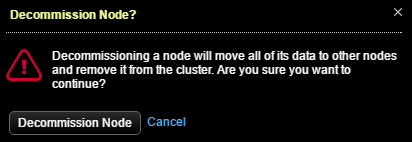
\includegraphics[width=0.75\textwidth]{img/4_installatie_cassandra/5_Remove_Node_3}
	\caption{Verwijderen van een node: Selecteer de node}
	\label{fig:cas_rem_3}
\end{figure}